\documentclass[sigconf]{acmart}
\synctex=1


% Copyright
%\setcopyright{none}
%\setcopyright{acmcopyright}
%\setcopyright{acmlicensed}
\setcopyright{rightsretained}
%\setcopyright{usgov}
%\setcopyright{usgovmixed}
%\setcopyright{cagov}
%\setcopyright{cagovmixed}


% DOI
\acmDOI{10.475/123_4}

% ISBN
\acmISBN{123-4567-24-567/08/06}

%Conference
%\acmConference[WOODSTOCK'97]{ACM Woodstock conference}{July 1997}{El
%  Paso, Texas USA}
%\acmYear{1997}
\copyrightyear{2016}



%=================================================================
% 
\newcount\DraftStatus  % 0 suppresses notes to selves in text
\DraftStatus=1   % TODO: set to 0 for final version
%=================================================================

%=================================================================
\usepackage{comment}
%=================================================================
%
\includecomment{JournalOnly}  
\includecomment{ConferenceOnly}  
\excludecomment{TulipStyle}
%
%=================================================================
%=================================================================
% gitlatexdiff
%
%  https://gitlab.com/git-latexdiff/git-latexdiff
%=================================================================
%  git latexdiff HEAD  HEAD~5 --main templatex.tex
%  git latexdiff HEAD~1  --main templatex.tex
%  View pdf to see difference
%
%=================================================================
%
% Todo Notes for marginal comments
% 
%\newcount\DraftStatus  % 0 suppresses notes to selves in text
%\DraftStatus=1   % TODO: set to 0 for final version
\ifnum\DraftStatus=1
	\usepackage[draft,colorinlistoftodos,color=orange!30]{todonotes}
\else
	\usepackage[disable,colorinlistoftodos,color=blue!30]{todonotes}
\fi 
%\usepackage[disable]{todonotes} % notes not showed
%\usepackage[draft]{todonotes}   % notes showed
%
\makeatletter
 \providecommand\@dotsep{5}
 \def\listtodoname{List of Todos}
 \def\listoftodos{\@starttoc{tdo}\listtodoname}
 \makeatother
%
%=================================================================
%
\usepackage{color}
\newcommand{\draftnote}[3]{ 
	\todo[author=#2,color=#1!30,size=\footnotesize]{\textsf{#3}}	}
% TODO: add yourself here:
%
\newcommand{\gangli}[1]{\draftnote{blue}{GLi:}{#1}}
\newcommand{\qwu}[1]{\draftnote{red}{QWu:}{#1}}
\newcommand{\gliMarker}
	{\todo[author=GLi,size=\tiny,inline,color=blue!40]
	{Gang Li has worked up to here.}}
\newcommand{\qwuMarker}
	{\todo[author=QWu,size=\tiny,inline,color=red!40]
	{Qiong Wu has worked up to here.}}
%=================================================================

%=================================================================
%
% general packages
%  https://en.wikibooks.org/wiki/Category:Book:LaTeX
%  https://en.wikibooks.org/wiki/LaTeX/Package_Reference
%
%=================================================================
\usepackage{graphicx}
\usepackage{algorithm}
\usepackage{algorithmic}
\usepackage{breqn}
\usepackage{subcaption}
\usepackage{multirow}
\usepackage{psfrag}
\usepackage{url}
\usepackage{hyperref}
%\usepackage[colorlinks]{hyperref}
%\usepackage{cite}
\usepackage{cleveref}
\usepackage{booktabs}
\usepackage{rotating}
\usepackage{colortbl}
\usepackage{paralist}
%\usepackage{geometry}
\usepackage{epstopdf}
\usepackage{nag}
\usepackage{microtype}
\usepackage{siunitx}
\usepackage{nicefrac}
% for random text
\usepackage{lipsum}
\usepackage[english]{babel}
\usepackage[pangram]{blindtext}
% for tikz figures
\usepackage{tikz}
\usetikzlibrary{fit,positioning,arrows.meta,shapes,arrows}
%\tikzset{neuron/.style={circle,thick,fill=black!25,minimum size=17pt,inner sep=0pt},
%	input neuron/.style={neuron, draw,thick, fill=gray!30},
%	hidden neuron/.style={neuron,fill=white,draw},
%	hoz/.style={rotate=-90}}
%
%=================================================================



\begin{TulipStyle}
\usepackage[numbers]{natbib}
%=================================================================
%
% Version control information
%
%=================================================================
\usepackage{gitinfo2}
%=================================================================
\usepackage{fancyhdr}
\pagestyle{fancy}
\fancyhead{} % clear all header fields
\fancyhead[RO,LE]{\textsl{\rightmark}}
\fancyhead[LO,RE]{\ensuremath{\Rightarrow}
		\textbf{\textbf{[CONFIDENTIAL]}}\ensuremath{\Leftarrow}}
\fancyhead[CO,CE]{}
%=================================================================
\fancyfoot{} % clear all footer fields
\fancyfoot[CE,CO]{\textbf{\thepage}} 
\fancyfoot[LO,LE]{
\includegraphics[height=.9\headheight]{logos/tulip-logo.eps}
		\gitVtagn-\gitBranch\ (\gitCommitterDate)}
\fancyfoot[RO,RE]{Committed by: \textsl{\gitCommitterName}}

\setlength{\headheight}{12pt}
\renewcommand{\headrulewidth}{0.4pt}
\renewcommand{\footrulewidth}{0.4pt}
%=================================================================


%=================================================================
% for math notations
% ----------------------------------------------------------------
\usepackage{mathtools}
\usepackage{amsthm}
%
% THEOREMS -------------------------------------------------------
%
\newtheorem{thm}{Theorem}[section]
\newtheorem{cor}[thm]{Corollary}
\newtheorem{lem}[thm]{Lemma}
\newtheorem{prop}[thm]{Proposition}
\theoremstyle{definition}
\newtheorem{defn}[thm]{Definition}
\theoremstyle{remark}
\newtheorem{rem}[thm]{Remark}
\numberwithin{equation}{section}
% MATH -----------------------------------------------------------
\newcommand{\norm}[1]{\left\Vert#1\right\Vert}
\newcommand{\abs}[1]{\left\vert#1\right\vert}
\newcommand{\set}[1]{\left\{#1\right\}}
\newcommand{\Real}{\mathbb R}
\newcommand{\eps}{\varepsilon}
\newcommand{\To}{\longrightarrow}
\newcommand{\BX}{\mathbf{B}(X)}
% ----------------------------------------------------------------
\newcommand{\I}{{\cal I}}
\newcommand{\Id}{{\cal I} }
\newcommand{\Dc}{{\cal D}}
\newcommand{\J}{{\cal J}}
\newcommand{\Dn}{{\cal D}_n}
\newcommand{\Dd}{{\cal D}_n }
\renewcommand{\P}{{\cal P}}
\newcommand{\Nu}{{\cal N} }
\newcommand{\B}{{\cal B}}
\newcommand{\Bf}{{\bf B}}
\newcommand{\Y}{{\bf Y}}
\newcommand{\A}{{\cal A}}
% ----------------------------------------------------------------
\newcommand{\V}{{\cal V}}
\newcommand{\M}{{\cal M}}
\newcommand{\F}{{\cal F}}
\newcommand{\Fd}{{\cal F}}
\newcommand{\BF}{{\cal BF}_n}
\newcommand{\BFd}{{\cal BF}_n}
\newcommand{\TF}{{\cal TF}_n}
\newcommand{\TFd}{{\cal TF}_n}
%\newcommand{\G}{{\cal G}}
\newcommand{\X}{{\cal X}}
\newcommand{\E}{{\cal E}}
\newcommand{\K}{{\cal K}}
\newcommand{\T}{{\cal T}_n}
\renewcommand{\H}{{\cal H}}
% ----------------------------------------------------------------
\newtheorem{Remark}{Remark}
\newtheorem{proposition}{Proposition}
\newtheorem{theorem}{Theorem}
\newtheorem{lemma}{Lemma}
\newtheorem{corollary}{Corollary}
\newtheorem{example}{Example}
\newtheorem{definition}{Definition}
\newtheorem{Algorithms}{Algorithm}
% ----------------------------------------------------------------
\newcommand{\bu}{{\mathbf 1} }
\newcommand{\bo}{{\mathbf 0} }
\newcommand{\N}{\mbox{{\sl l}}\!\mbox{{\sl N}}}
% ----------------------------------------------------------------
\def\uint{[0,1]}
\def\proof{{\scshape Proof}. \ignorespaces}
\def\endproof{{\hfill \vbox{\hrule\hbox{%
   \vrule height1.3ex\hskip1.0ex\vrule}\hrule
  }}\par}
%
%=================================================================

\hypersetup
{
    pdfauthor={\gitAuthorName},
    pdfsubject={TULIP Lab},
    pdftitle={},
    pdfkeywords={TULIP Lab, Data Science},
%	bookmarks=true,  
}

\end{TulipStyle}




%=================================================================
%
\begin{document}
%
%=================================================================
% Preamble which will need to be changed for submission
%
\title{Title of This Paper}%
\titlenote{Produces the permission block, and
  copyright information}
\subtitle{What is my Subtitle?}
\subtitlenote{The full version of the author's guide is available as
  \texttt{acmart.pdf} document}


\author{Ben Trovato}
\authornote{Dr.~Trovato insisted his name be first.}
\orcid{1234-5678-9012}
\affiliation{%
  \institution{Institute for Clarity in Documentation}
  \streetaddress{P.O. Box 1212}
  \city{Dublin}
  \state{Ohio}
  \postcode{43017-6221}
}
\email{trovato@corporation.com}

\author{Gang Li}
\authornote{Corresponding Author}
\affiliation{%
  \institution{Deakin University}
  \city{Geelong, VIC 3216}
  \country{Australia}}
\email{gang.li@deakin.edu.au}

% The default list of authors is too long for headers.
\renewcommand{\shortauthors}{G. Li et al.}


\begin{abstract}
The abstract will be put here, ....
\end{abstract}

\keywords{ACM proceedings, \LaTeX, text tagging}

\maketitle

%=================================================================

%=================================================================
\section{Introduction}
\label{sec-intro}
In 2018, film revenue has increased significantly, and the film industry is more popular than ever.
What kind of movies make high box office receipts. In the process of preparation and shooting, 
whether the budget, the number of directors and actors have a great impact. Whether the publicity and 
preview of later films will affect the final box office income of films.

Data Analysis aims to show the relationship between attributes and box office revenue 
according to the data provided. And further integration of data, delete irrelevant data, 
unified data values and so on.

Models and Forecasts aims to use the integrated data to train the relevant models, 
improve the accuracy, and make the box office revenue forecast for some of the given data.

In this paper, we train the random forest model with the integrated data, 
and use the model to predict the box office of movies.
\section{Preliminaries} \label{sec-preliminaries}
Analyze the data in the preparation stage, and analyze it from different angles and box office. 
For example, from the perspective of budget, the number of actors, the number of crew members, 
and post-promotion. It also showcases popular movie genres and movie language in the form of a word cloud.


%\begin{center}
%  \begin{minipage}{0.3\linewidth}
%  \centering
%    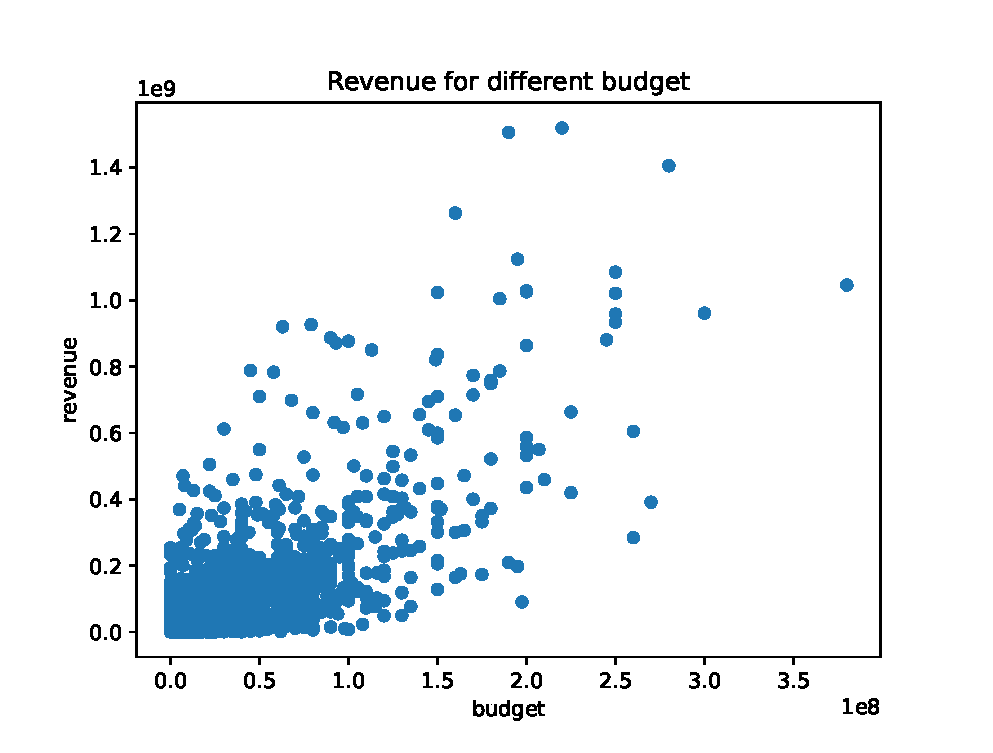
\includegraphics[width=0.8\linewidth]{figures//budget.eps}
%  {\small{Budget}}
%  \end{minipage}
%  \hfill
%  \begin{minipage}{0.3\linewidth}
%  \centering
%    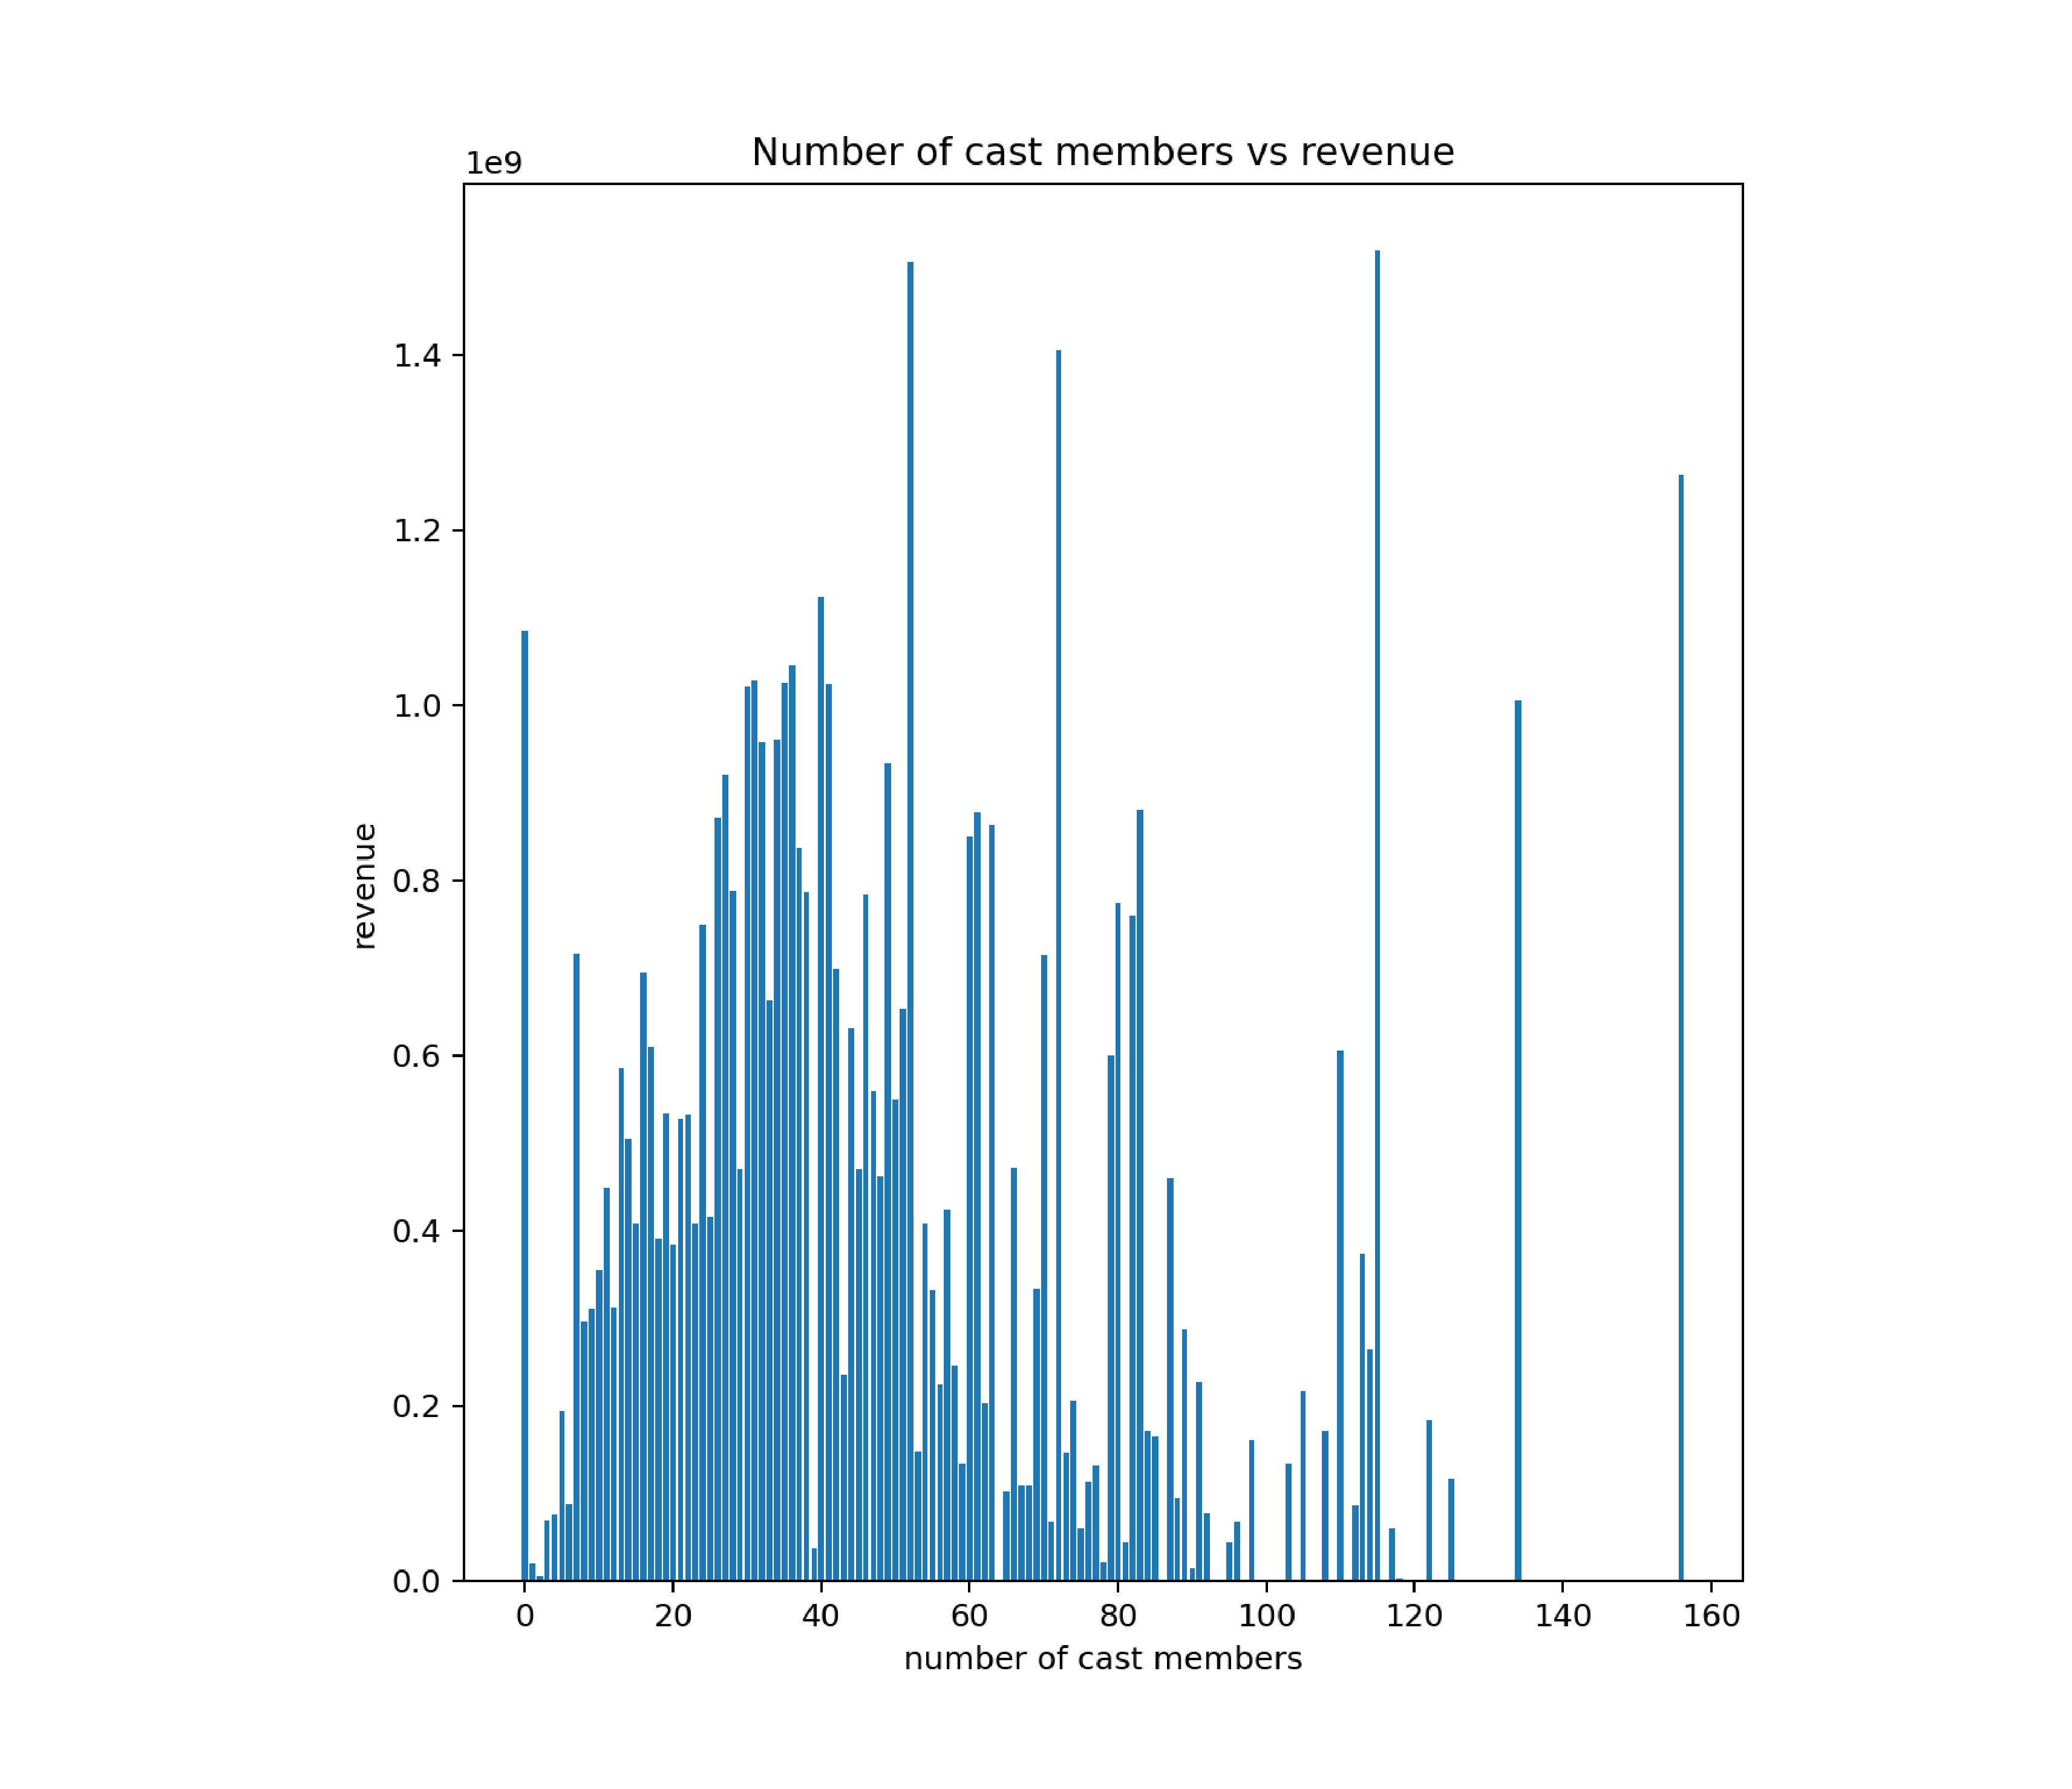
\includegraphics[width=0.8\linewidth]{figures//cest.eps}\\
%  {\small{Cast}}
%  \end{minipage}
%  \hfill
%  \begin{minipage}{0.3\linewidth}
%  \centering
%    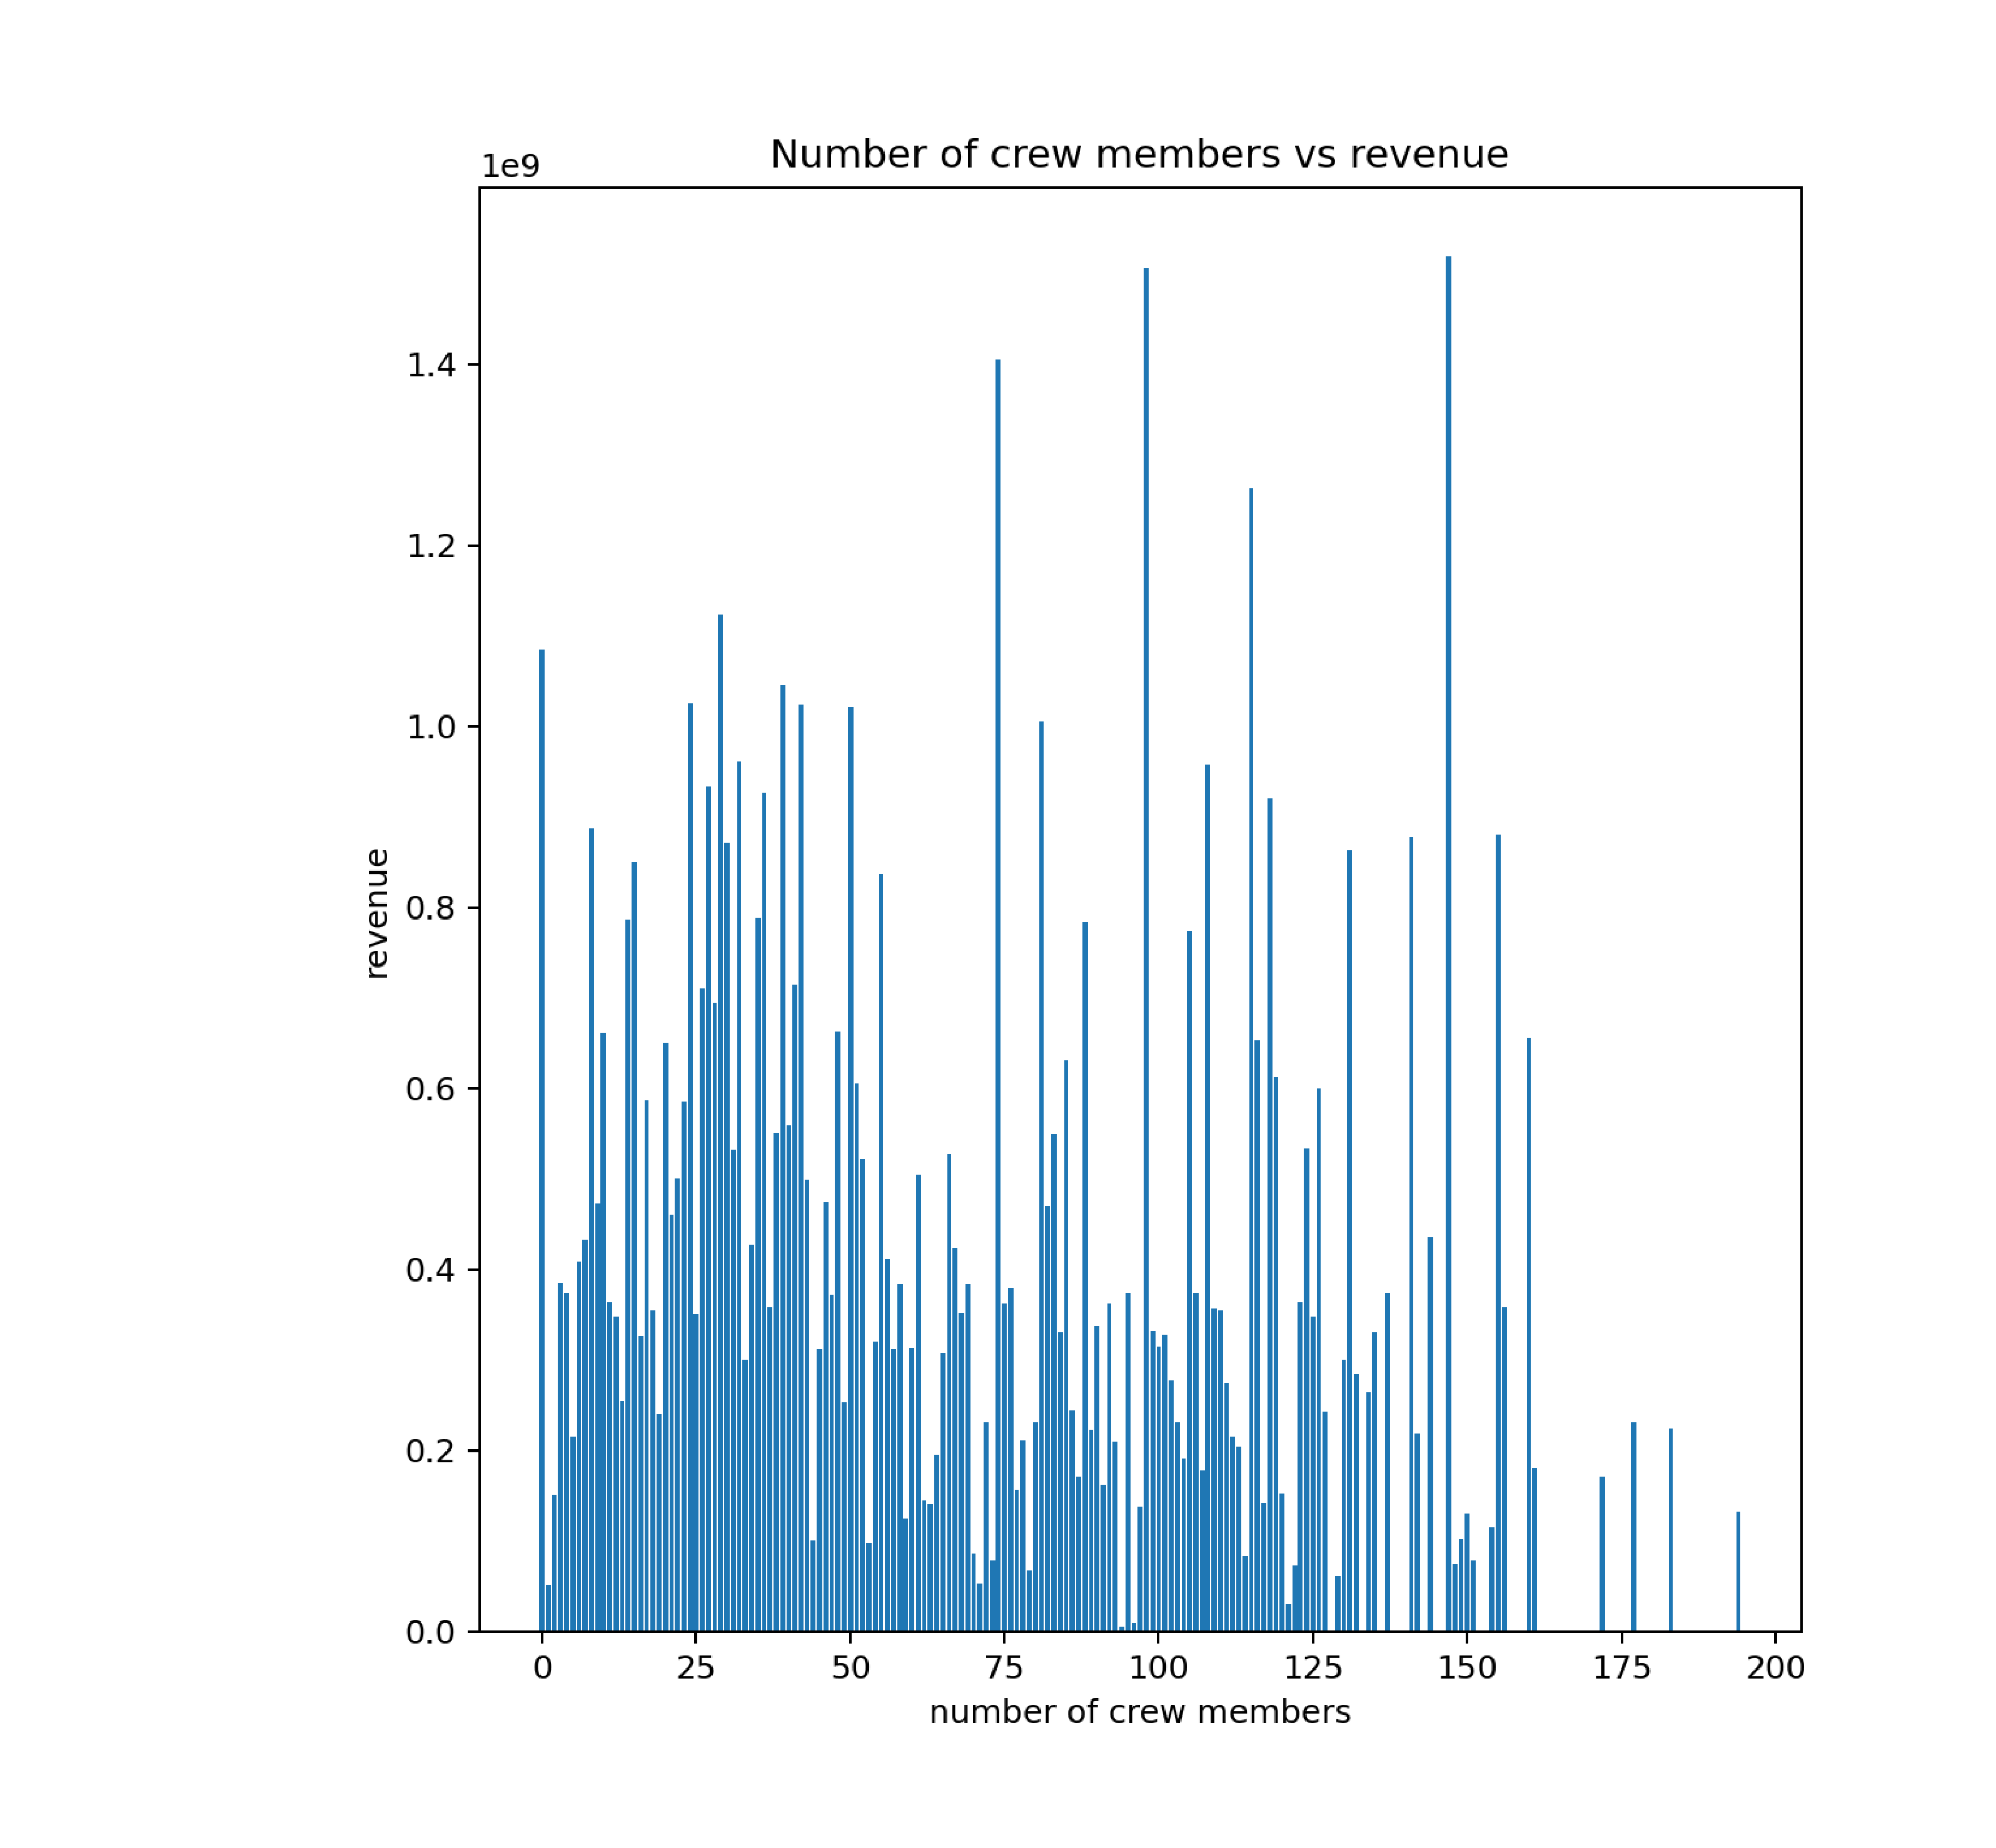
\includegraphics[width=0.8\linewidth]{figures//crew.eps}\\
%  {\small{Crew}}
%  \end{minipage}
%\end{center}


%\begin{center}
%  \begin{minipage}{0.3\linewidth}
%  \centering
%    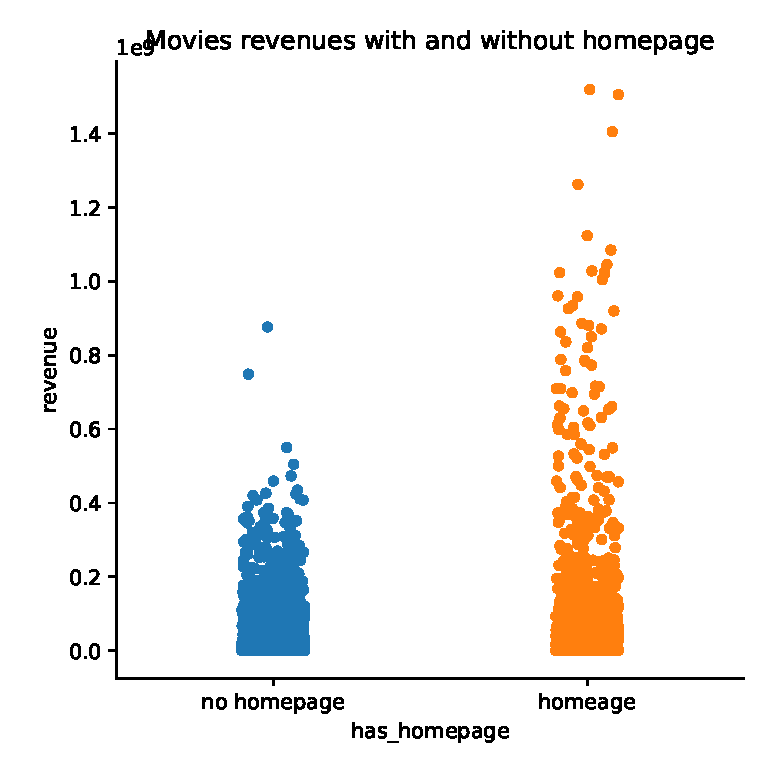
\includegraphics[width=0.8\linewidth]{figures//has_homepage.eps}
%  {\small{Homepage}}
%  \end{minipage}
%  \hfill
%  \begin{minipage}{0.3\linewidth}
%  \centering
%    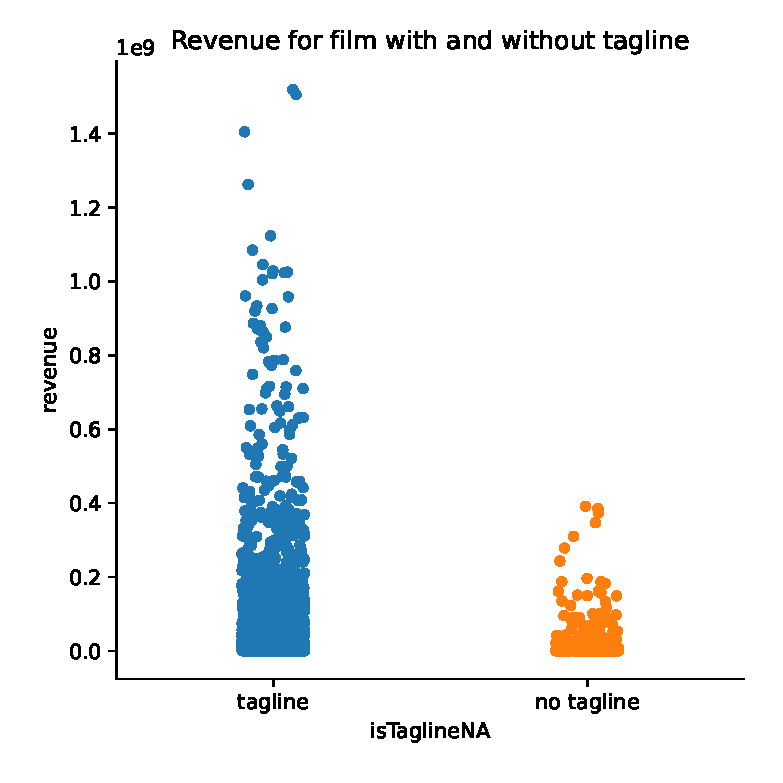
\includegraphics[width=0.8\linewidth]{figures//isTanglineNA.eps}
%  {\small{Tagline}}
%  \end{minipage}
%  \hfill
%  \begin{minipage}{0.3\linewidth}
%  \centering
%    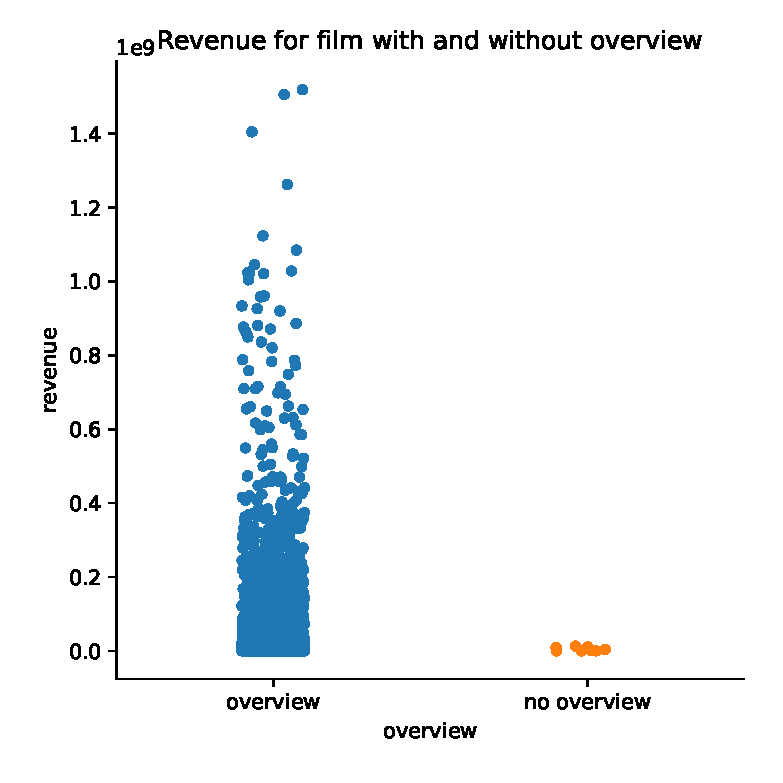
\includegraphics[width=0.8\linewidth]{figures//overview.eps}
%  {\small{Overview}}
%  \end{minipage}
%\end{center}

%\begin{center}
%  \begin{minipage}{0.3\linewidth}
%  \centering
%    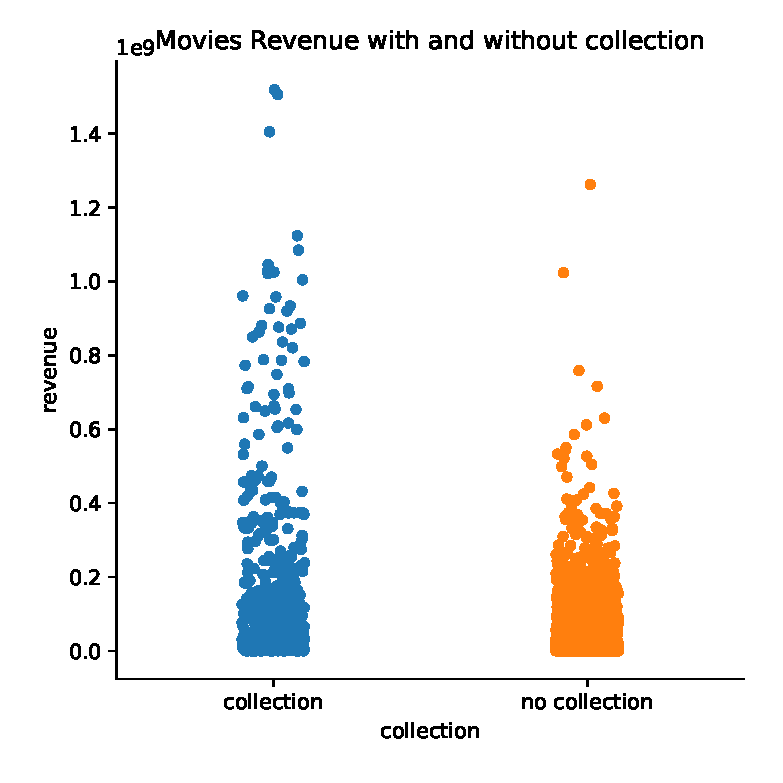
\includegraphics[width=0.8\linewidth]{figures//collection.eps}\\
%  {\small{File Series}}
%  \end{minipage}
%  \hfill
%  \begin{minipage}{0.3\linewidth}
%  \centering
%    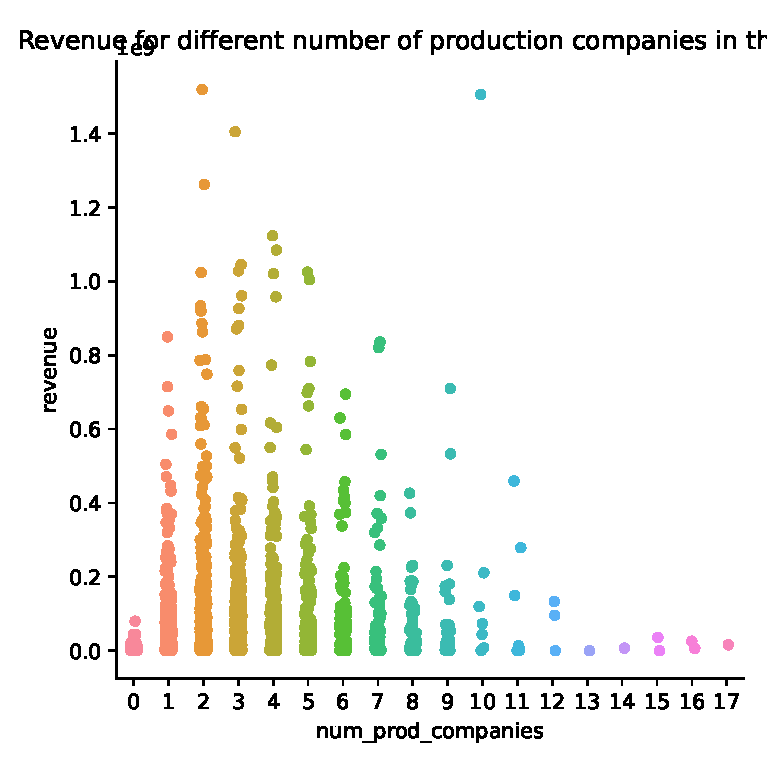
\includegraphics[width=0.8\linewidth]{figures//company.eps}\\
%  {\small{File Company}}
%  \end{minipage}
%  \hfill
%  \begin{minipage}{0.3\linewidth}
%  \centering
%    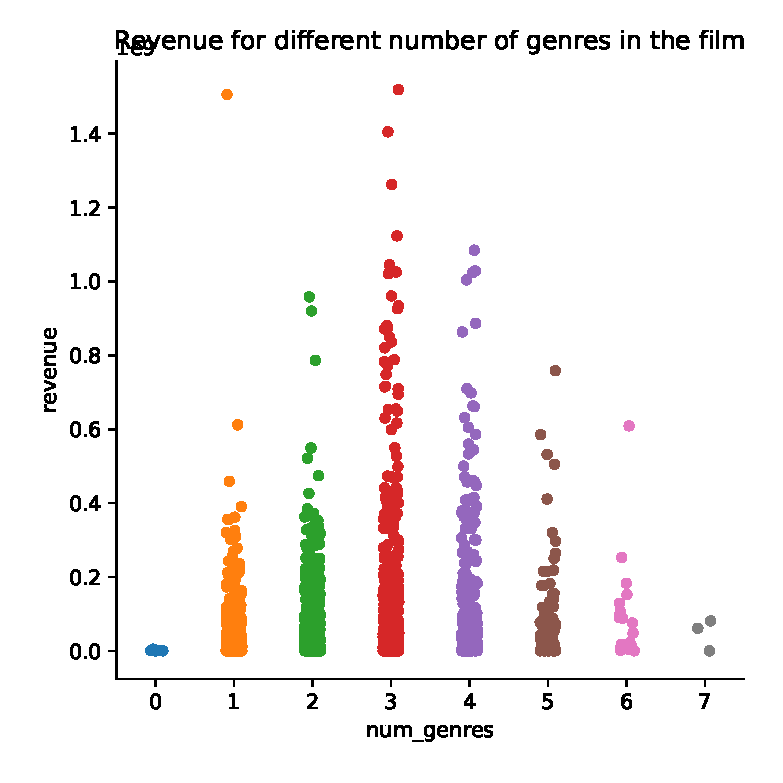
\includegraphics[width=0.8\linewidth]{figures//counrty.eps}
%  {\small{Company Number}}
%  \end{minipage}
%\end{center}


%\begin{center}
%  \begin{minipage}{0.4\linewidth}
%  \centering
%    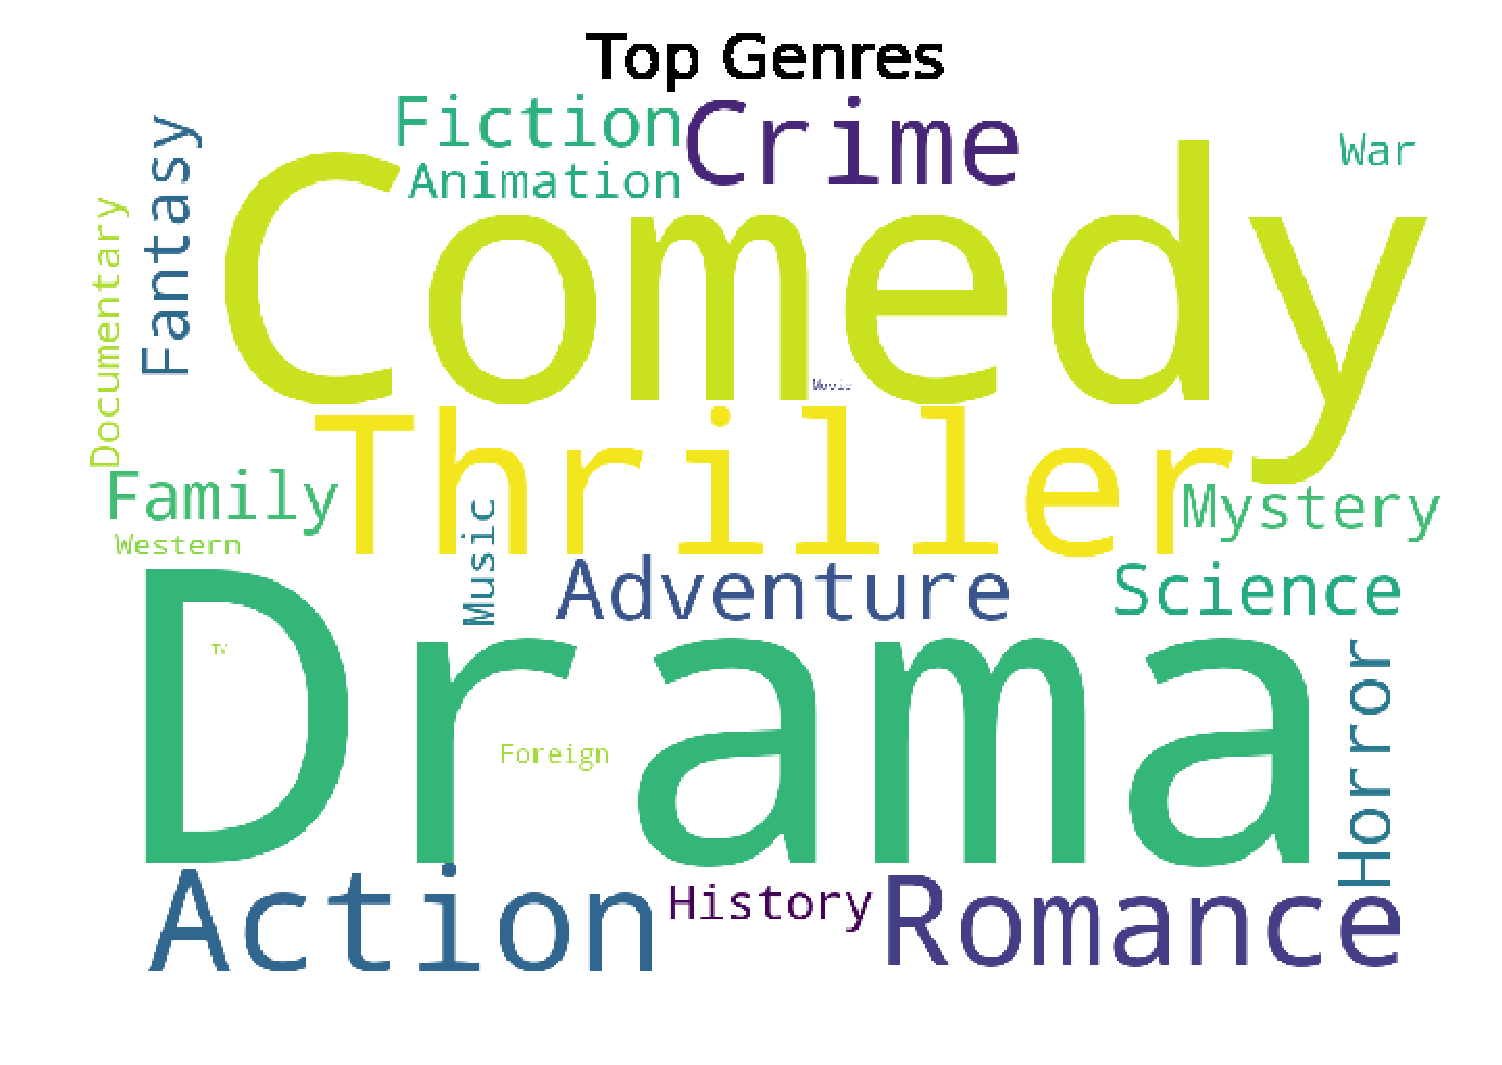
\includegraphics[width=0.8\linewidth]{figures//genre_clold.eps}\\
%  {\small{Genre}}
%  \end{minipage}
%  \hfill
%  \begin{minipage}{0.4\linewidth}
%  \centering
%    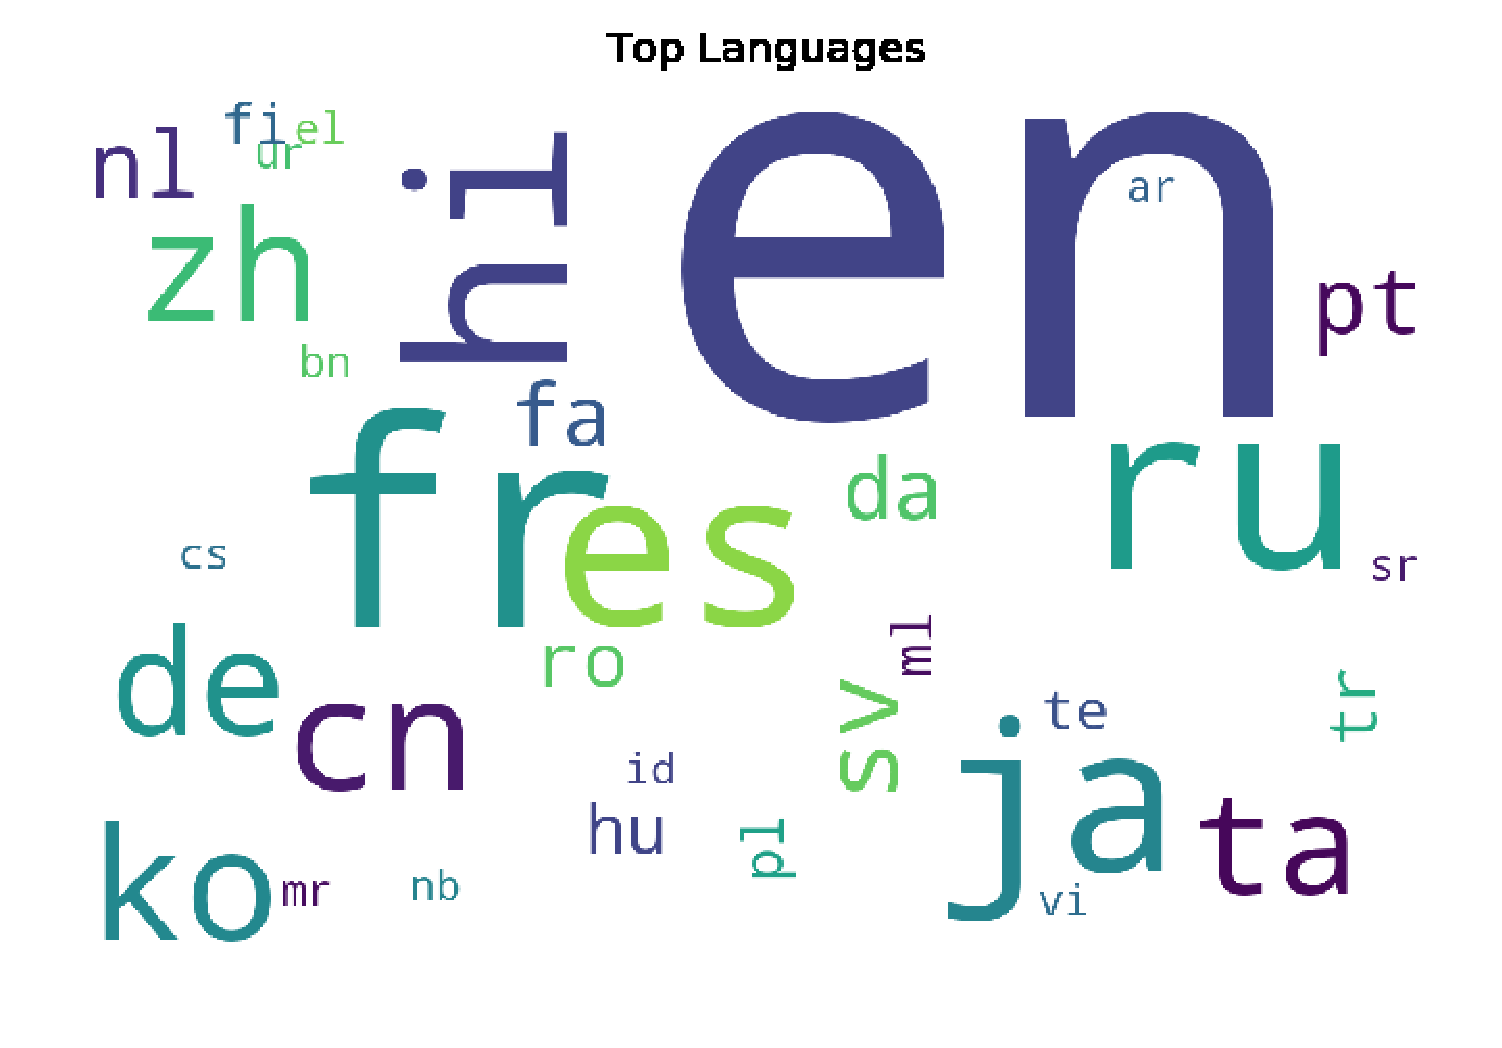
\includegraphics[width=0.8\linewidth]{figures//language.eps}\\
%  {\small{Language}}
%  \end{minipage}
%  \hfill
%\end{center}

\section{Method} \label{sec-method}
After the preparation work is completed, the data will be further processed. 
Delete data not related to the box office, For example: imdb_id, orginal_title, poster_path, status.
Normalize some data,For example: has_homepage, collection, overview, isTaglineNA, Keywords_count etc

%5\begin{table}
%  \begin{center}
%    \centering
%    \caption{Partial Processing Data}
%    \begin{tabular}{ c | c }
%      \toprule
%      Name     &  Description        \\
%      \midrule
%      imdb id       &  ID of movie in TMDB  \\
%      orginal title &  The original name of the movie \\
%      poster path &  Movie poster link \\
%      status   & The state of the film \\
%      keywords      &  Key words of movies \\
%      tagline &  The slogan of the film \\
%      homepage & Official film Homepage \\
%      overview   &A brief description of the film \\
%      collection & Series name of film series\\
%      release date & Film release time\\ 
%      \bottomrule
%      \end{tabular}
%  \end{center}
%\end{table}

After the completion of data processing, the model was established using random forest algorithm.

Random Forest Algorithm is an ensemble technique that combines multiple decision trees. 
    Other advantages of random forests are that they are less sensitive to outliers in the dataset 
    and don’t require much parameter tuning.

%\section{Experiment} \label{sec-experiment}
%After the training of the model, the prediction was made by using the data.

\section{Conclusions} \label{sec-conclusions}
The investment in the early stage and publicity in the later stage have an impact on the box office.

In the early stage, the number of actors and crew should be moderate, not the more the better.

The prediction accuracy can be further improved, such as using XGBoost.
\section*{Acknowledgment}

Thanks for the learning opportunities provided by Tulip, 
I grew up rapidly in this period of time. 
Thanks to my tutor for answering questions and puzzles during my study, 
which is my rapid progress. At the same time, I should also like to thank my senior brother, 
sister and classmates for their help. When I am not successful in my study, 
I will lend a helping hand to help me solve problems.

% ----------------------------------------------------------------
\bibliography{tuliplab,yourbib}
\bibliographystyle{ACM-Reference-Format}
%=================================================================

\end{document}

